\section{Results}

In the following sections we will discuss some key results;
for a more complete look at the output of the scripts, we ask that you please
consult the Appendices.

\subsection{Teleportation}

The main result of the teleportation protocol is summarized in Fig.
\ref{fig:teleport_histogram}. The ideal simulation fidelities are all within
statistical error of unity, an important check to ensure that the state,
reconstructed through tomography and post-measurement selection scheme both are
working as expected. The Noisy Simulator is modelled using the single-qubit
errors, CNOT errors and a model of readout error with symmetric bit flip
probabilities in each backend \cite{qiskit_org}. As we will continue to see with
the other circuits, the noise model tends to overestimates the performance of
the backend, but interestingly in this case, for the Melbourne device, we find
that the noise model almost matches that of the device.

\begin{figure}[h!] \centering
	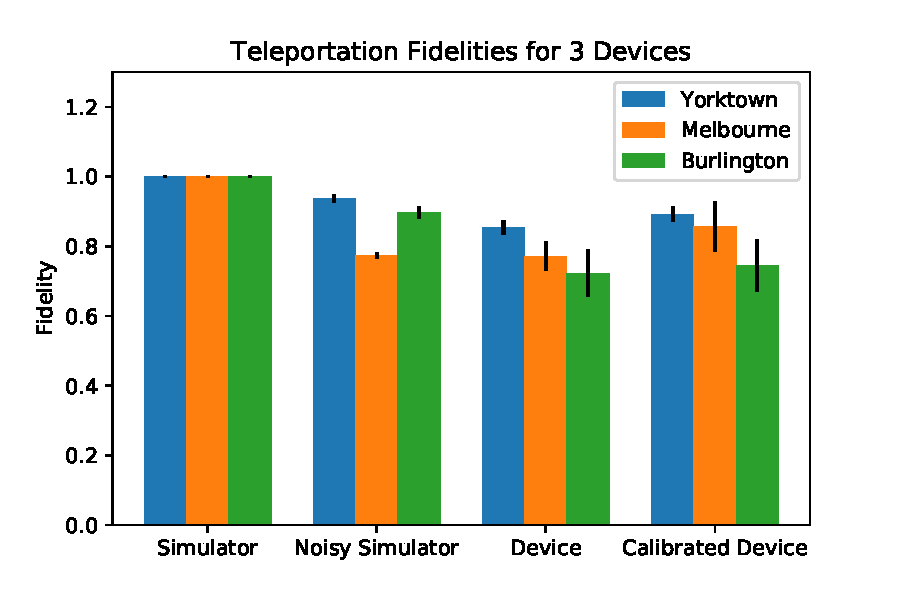
\includegraphics[width=0.48\textwidth]{images/results/teleport_histogram.pdf}
	\caption{Fidelity results for the Teleportation protocol. Error bars, showing
one standard deviation, are estimated by taking the variance over 15 runs of
8,192 shots each (a total of 122,880 shots). All simulation fidelities are
within statistical error of unity.}
	\label{fig:teleport_histogram}
\end{figure}
The noise model captures the error in the Burlington device much less
accurately. We would expect that Burlington would perform almost as well as
Yorktown from the estimates on the noisy simulator, but in fact it performs the
worst of the three. We suspect, as will be seen again below for the other
circuits, that this is a consequence of the number of gates needed to implement
the circuit on the real device.

\begin{figure}[h!]
  \begin{subfigure}{.5\textwidth}
    \centering
    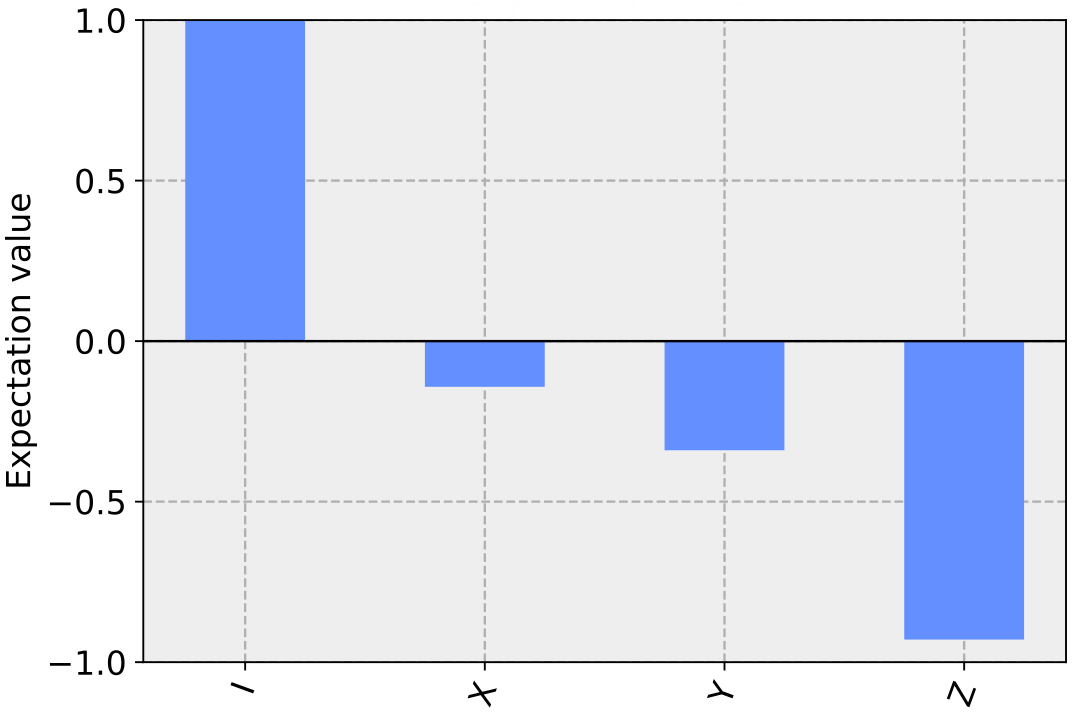
\includegraphics[width=.8\linewidth]{images/results/tele_pauli_sim.png}
    \caption{The expected Pauli set.}
    \label{fig:tele_pauli_sim}
  \end{subfigure}
  \newline
  \begin{subfigure}{.5\textwidth}
    \centering
    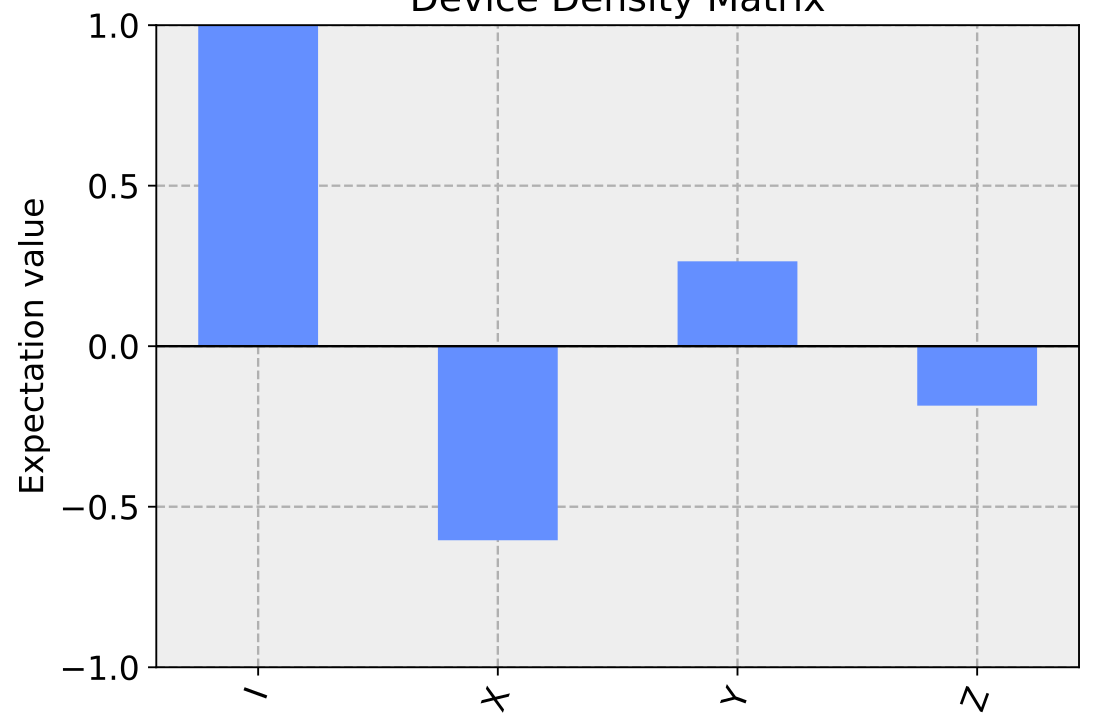
\includegraphics[width=.8\linewidth]{images/results/tele_pauli_dev.png}
    \caption{The output Pauli set for the device.}
    \label{fig:tele_pauli_dev}
  \end{subfigure}
  \newline
  \begin{subfigure}{.5\textwidth}
    \centering
    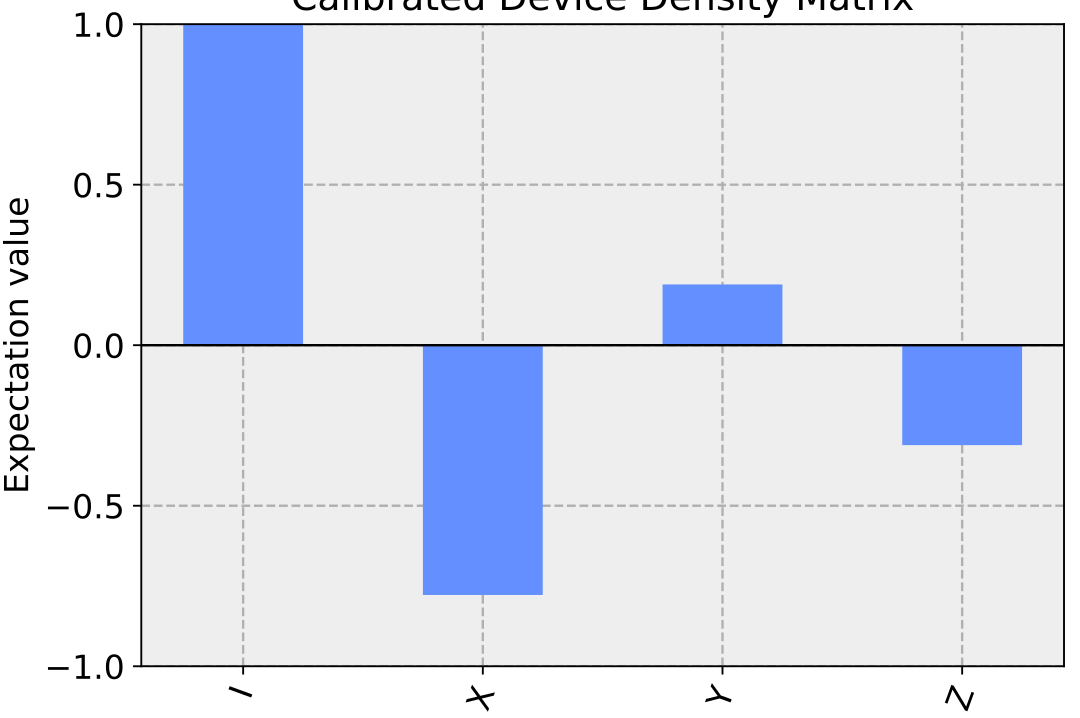
\includegraphics[width=.8\linewidth]{images/results/tele_pauli_cal.png}
    \caption{The calibrated device Pauli set.}
    \label{fig:tele_pauli_dev}
  \end{subfigure}
  \caption{The expectation values match those we expect after calibrating for
readout error. Errors in measurement contribute greatly to the low fidelity of
our final states. The type of correction seen in the figures above accounts for
the increased fidelity for the calibrated device in Fig.
\ref{fig:teleport_histogram}. Data plotted here is taken for 8192 shots on the
Melbourne backend.}
  \label{fig:tele_paulis}
\end{figure}

In order to check the readout calibration, it is useful to compare Pauli sets of
the different outcomes, which we can see in Fig. \ref{fig:tele_paulis}. These
plots make the expectation values of the three measurement bases very visible,
which eases the comparison of the results. Though not perfect, the output
calibrated for readout error fits the expected state much better than the
original device output. We can conclude from this that indeed, a large source of
error in the system comes from measurement, and the state the circuit actually
creates is much better than what we would naively assume through tomography
alone!

% This thing here is to test a full size picture don't delete.
% \begin{figure*}
%   \centering
%   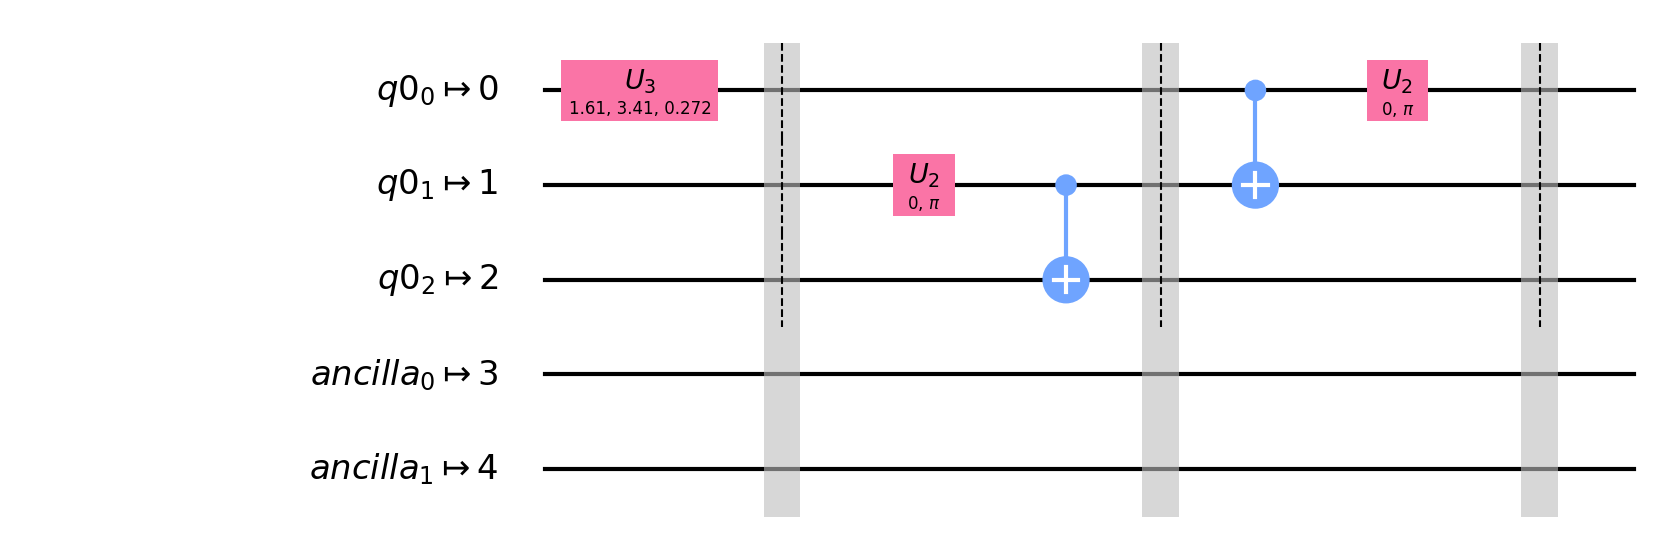
\includegraphics[width=\textwidth]{images/teleport_ibmqx2.png}
%   \caption{The most densely connected 5-qubit device at IBM Q. As we will see,
%     equally as important as the single-qubit and CNOT error rates is the degree of
%     connectivity in a device. Figure from \cite{ibmq_yorktown}.}
%   \label{fig:yorktown_connections}
% \end{figure*}

\subsection{Entanglement Swapping}

We now turn to Entanglement Swapping, a protocol largely similar to
teleportation, in that it teleports one half of an entangled pair. The main
result can be found in Fig. \ref{fig:swap_histogram}. The swapping protocol was
implemented for initial states (that is, the top two qubits, the bottom two were
always prepared in $\ket{\Phi^+}$) that were not, in general, Bell states, but
instead states with some degree of entanglement. We felt this was important in
order to probe our ability to reconstruct arbitrary states using tomography, and
show that indeed the swapping protocol should work for any entangled pair.

\begin{figure}[h!]
  \centering
  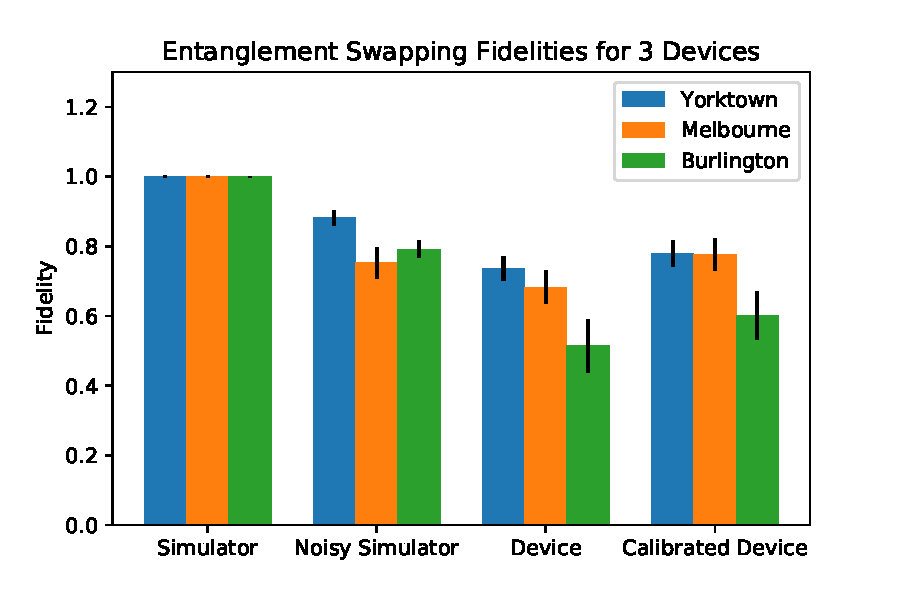
\includegraphics[width=0.48\textwidth]{images/results/swap_histogram.pdf}
	\caption{Fidelity results for the Entanglement Swapping protocol. Error bars
are estimated by taking the variance over 15 runs of 8,192 shots each (a total
of 122,880 shots).}
	\label{fig:swap_histogram}
\end{figure}

Again we see that the simulation fidelities are 1 within
statistical error, which means that the swapping of initial Bell-states are done
correctly using tomography to construct the final state, and post-measurement
selection to transform specified results to specific basis. As we expected,
fidelities from the noisy simulator are much better than results from all the
devices.

\begin{figure}[h!]
	\begin{subfigure}{.5\textwidth} \centering % include first image
		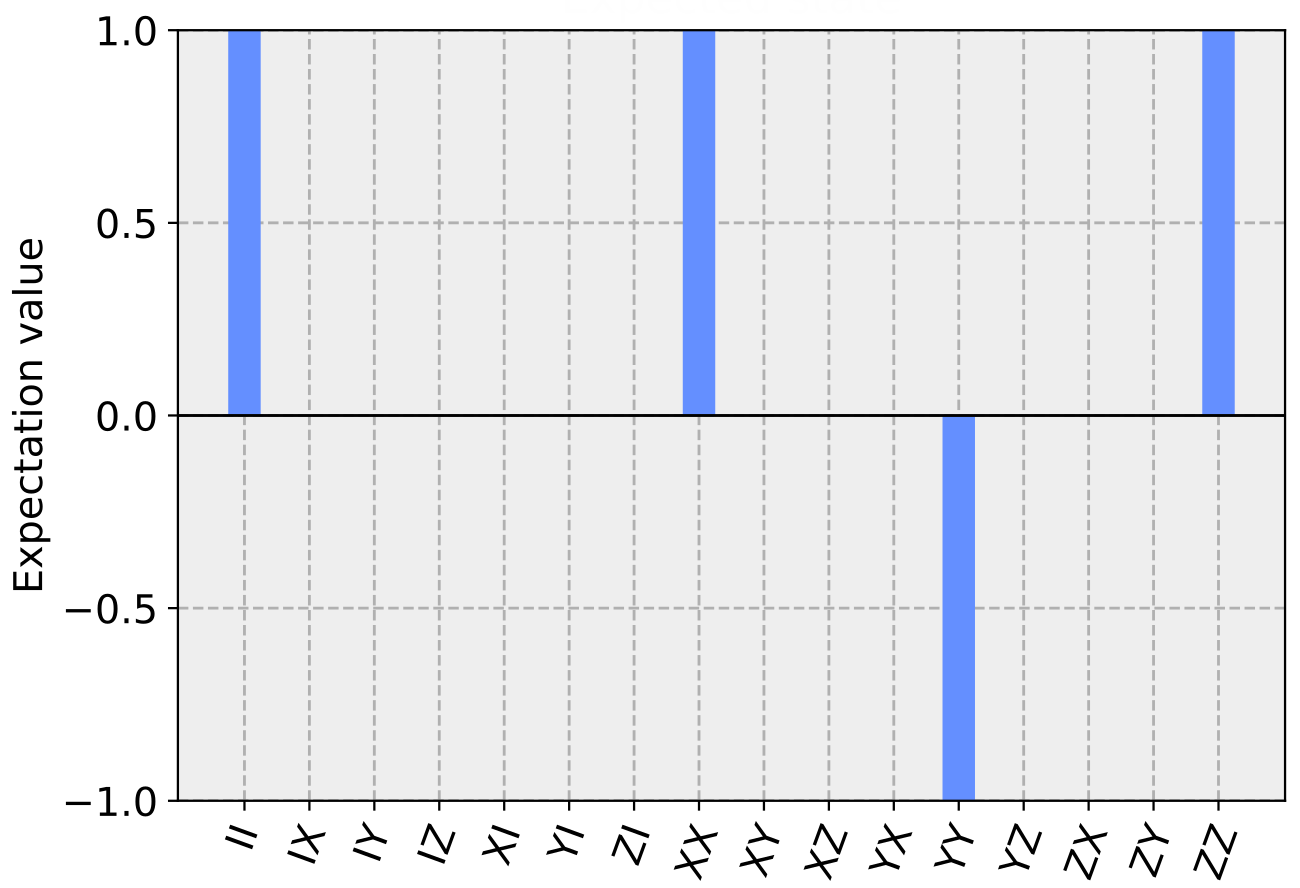
\includegraphics[width=.8\linewidth]{images/results/swap_pauli_sim.png}
		\caption{The expected Pauli set.}
		\label{fig:swap_pauli_sim}
	\end{subfigure} \newline
	\begin{subfigure}{.5\textwidth} \centering % include second image
		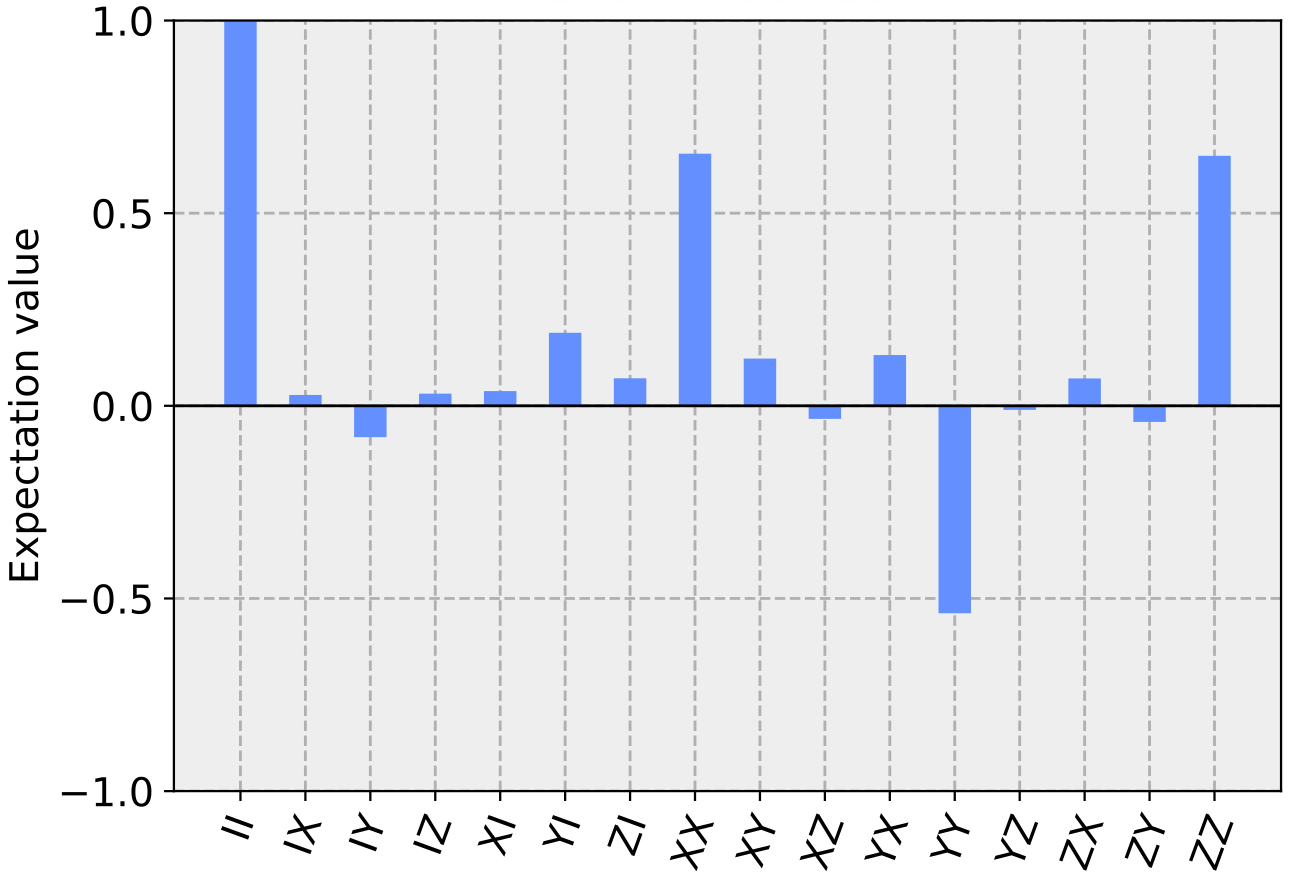
\includegraphics[width=.8\linewidth]{images/results/swap_pauli_dev.png}
		\caption{The output Pauli set for the device.}
		\label{fig:swap_pauli_dev}
	\end{subfigure} \newline
	\begin{subfigure}{.5\textwidth} \centering % include second image
		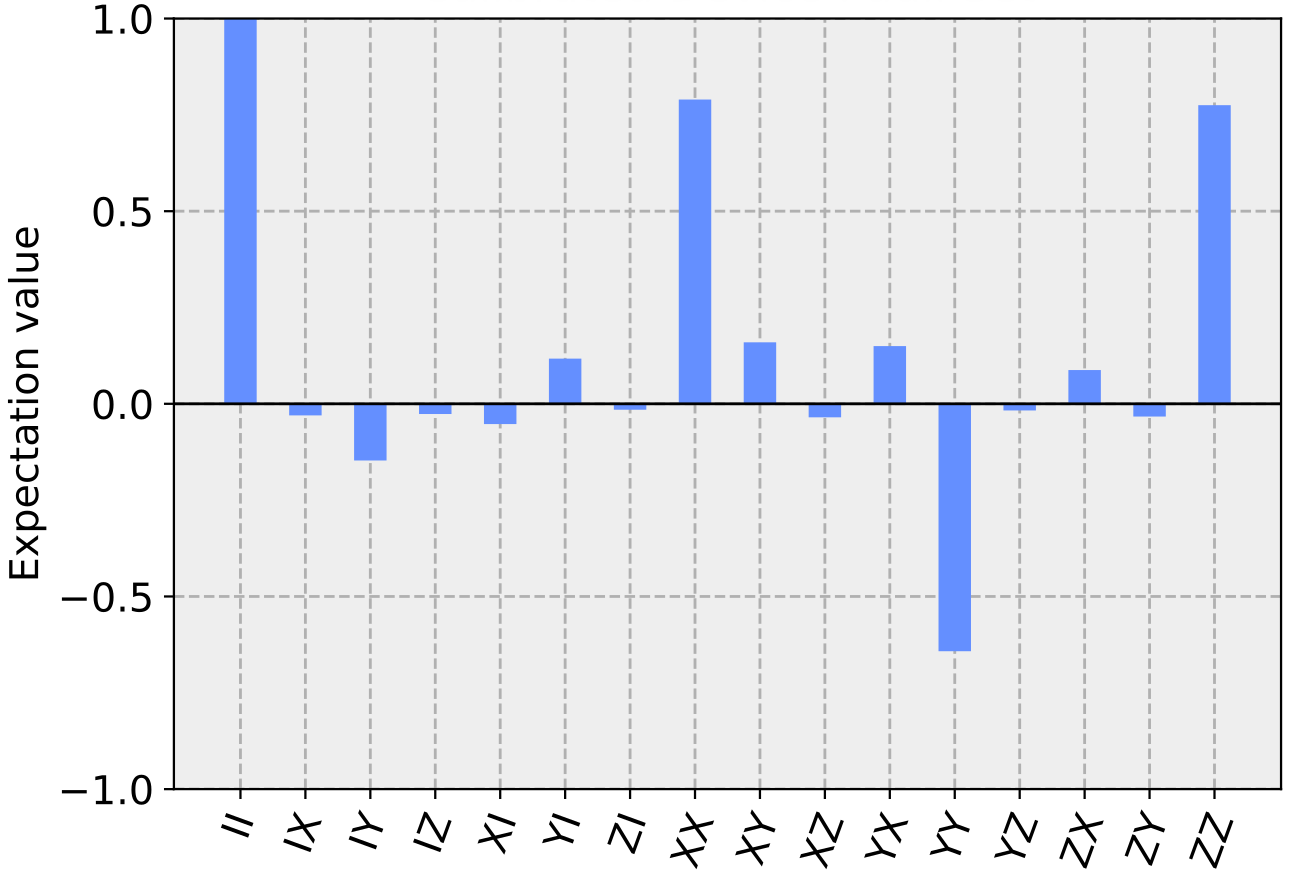
\includegraphics[width=.8\linewidth]{images/results/swap_pauli_cal.png}
		\caption{The calibrated device Pauli set.}
		\label{fig:swap_pauli_dev}
	\end{subfigure}
	\caption{ Pauli set entanglement swapping results for the ideal simulator, the
		device and the calibrated device. The type of correction seen in the figures
		above accounts for the increased fidelity for the calibrated device in Fig.
		\ref{fig:swap_histogram}. Data plotted here is taken for 8192 shots on the
		Melbourne backend.}
	\label{fig:swap_paulis}
\end{figure}
\newpage
Burlington's device performance is again much worse than would be
expected from the noisy simulator results. We can appreciate this decline by
comparing the number of gates needed to implement swap on Burlington to those
numbers for Melbourne and Yorktown. Where the former requires 9 CNOT gates to
implement the protocol on its T-shaped circuitry, the latter two require the
minimum of just three. This has huge impact on the output, and places the
backend with the highest single-qubit U$_2$ and CNOT fidelities in last place
when it comes to implementing swap. 

\begin{figure}[h]
	\begin{subfigure}{.5\textwidth}
    \centering
		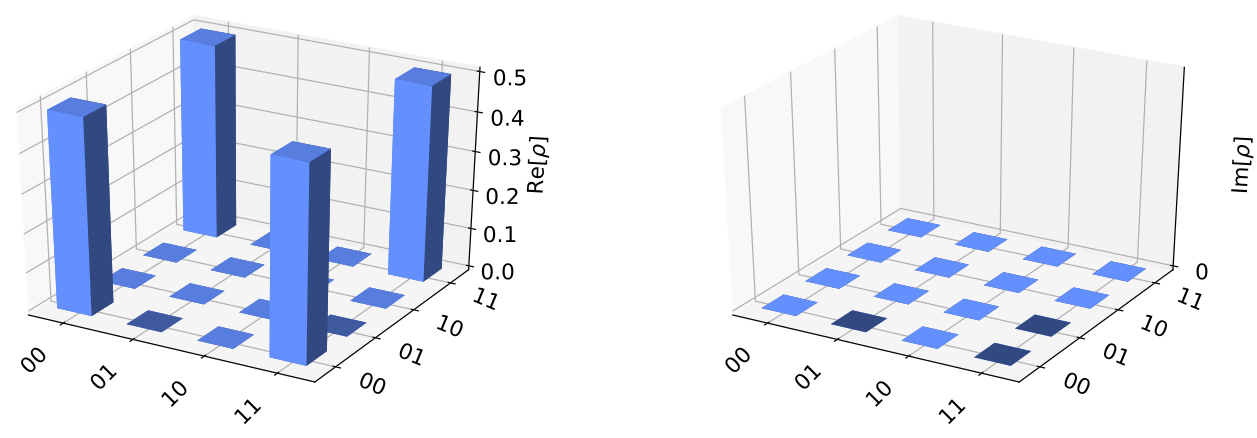
\includegraphics[width=.8\linewidth]{images/results/swap_density_sim.png}
		\caption{The expected Density matrix.}
		\label{fig:swap_density_sim}
	\end{subfigure} \newline
	\begin{subfigure}{.5\textwidth}
    \centering
		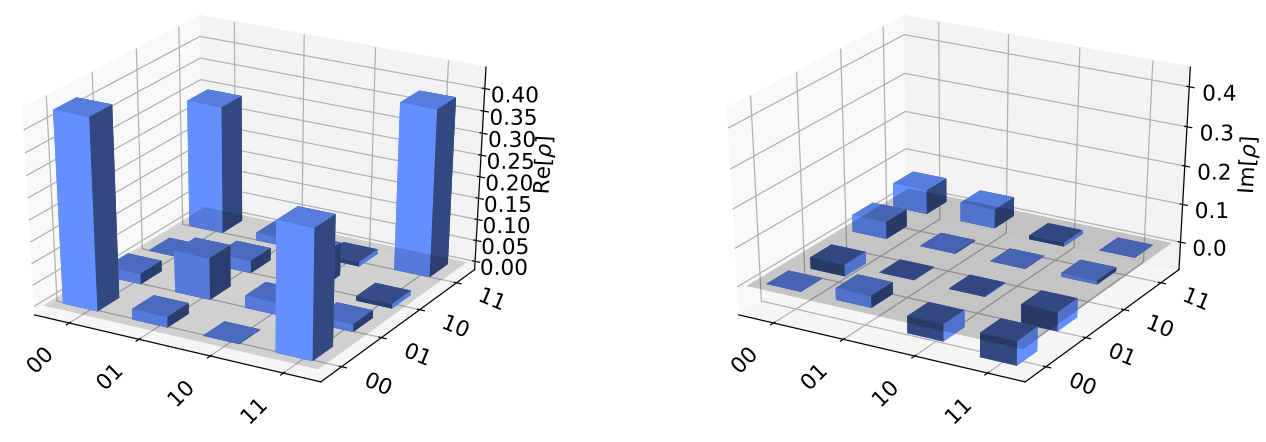
\includegraphics[width=.8\linewidth]{images/results/swap_density_dev.png}
		\caption{The output Density matrix for the device.}
		\label{fig:swap_density_dev}
	\end{subfigure} \newline
	\begin{subfigure}{.5\textwidth}
    \centering
		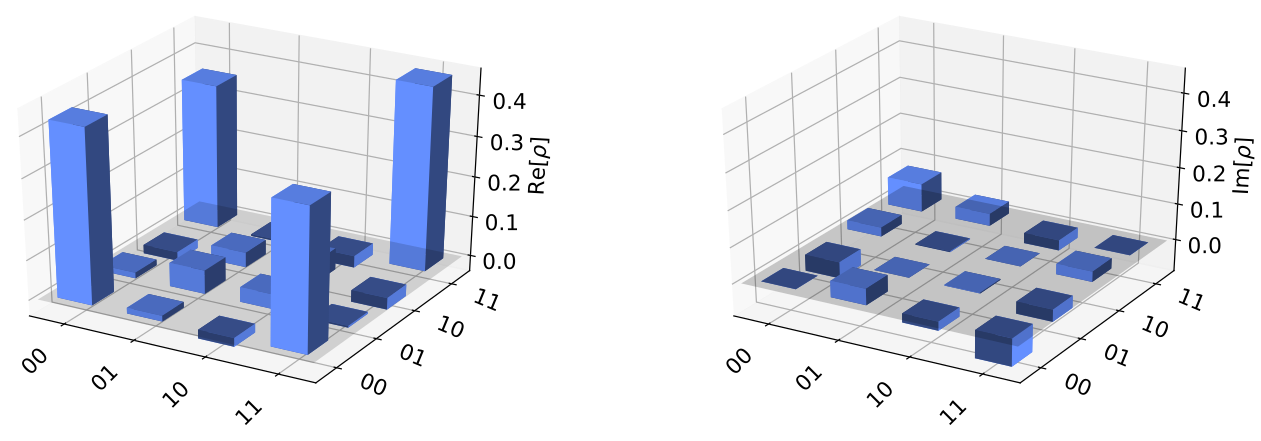
\includegraphics[width=.8\linewidth]{images/results/swap_density_cal.png}
		\caption{The calibrated device Density matrix.}
		\label{fig:swap_density_dev}
	\end{subfigure}
	\caption{ The entanglement swapping density matrices for the ideal simulator,
    the device and the calibrated device. Data plotted here is taken for 8192 shots
    on the Melbourne backend. }
	\label{fig:swap_density}
\end{figure}

In order to appreciate the effect of readout calibration on the output, we show,
in Fig. \ref{fig:swap_paulis}, the Pauli sets for an entanglement swapping
circuit that takes both input pairs as $\ket{\Phi^+}$. We chose this for our
plots as it is particularly easy, with a Bell state, to know what it is we
expect from the plots. We expect, of course, large values for the
$\langle XX \rangle$, $\langle YY \rangle$, $\langle ZZ \rangle$, and otherwise
very small values, as seen in Fig. \ref{fig:swap_pauli_sim}. The readout
calibration does a decent job of boosting the like-like correlations, as can
also be seen from Fig. \ref{fig:swap_density}.

\subsection{Entanglement Purification}


\subsection{Grover's Algorithm}


%%% Local Variables:
%%% mode: latex
%%% TeX-master: "report"
%%% End: